%% LyX 2.4.4 created this file.  For more info, see https://www.lyx.org/.
%% Do not edit unless you really know what you are doing.
\documentclass[dutch]{article}
\usepackage[T1]{fontenc}
\usepackage[utf8]{inputenc}
\usepackage{color}
\usepackage{float}
\usepackage{amstext}
\usepackage{graphicx}
\usepackage{geometry}
\geometry{verbose,tmargin=1in,bmargin=1in,lmargin=1in,rmargin=1in}

\makeatletter
%%%%%%%%%%%%%%%%%%%%%%%%%%%%%% User specified LaTeX commands.
%\usepackage{epstopdf} % to include .eps graphics files with pdfLaTeX
\usepackage{flafter}   % Don't place floats before their definition
%\usepackage{topcapt}  % Define \topcation for placing captions above tables (not in gwTeX)

\usepackage{xurl}      % better URL setting, uses old url package

\usepackage{xcolor}
\definecolor{darkblue}{rgb}{0,0,0.4}
\usepackage[]{hyperref} % Generates all cross references
\hypersetup{            % Setting options for hyperref package
	breaklinks=true,    % break line with long hyperlinks
	colorlinks=true,    % coloured links
	linkcolor=blue,
	filecolor=magenta,
	urlcolor=darkblue,
	citecolor=blue,
	backref=page
} 

\usepackage{memhfixc}  % remove conflict between the memoir class & hyperref
\usepackage{pdfsync}   % enable tex source and pdf output syncronicity

\usepackage{memhfixc}  % remove conflict between the memoir class & hyperref
\usepackage{pdfsync}   % enable tex source and pdf output syncronicity

\usepackage{alltt}

% \usepackage{listings}
% \usepackage{xcolor}

% \lstdefinestyle{mystyle}{
%   language=Python,
%   numbers=left
% }

% Put lstset here, after lstdefinestyle
% \lstset{style=mystyle}

\makeatother

\usepackage{babel}
\usepackage{listings}
\lstset{language=Python,
extendedchars=false,
frameround=fttt,
numbers=left,
% line numbers use none,
numberstyle={\tiny},
stepnumber=2,
% line numbers only every so many,
numbersep=9pt,
% how far line numbers from text?,
showspaces=false,
showstringspaces=false,
showtabs=false,
tab={\rightarrowfill},
basicstyle={\small},
keywordstyle={\color{blue}},
commentstyle={\color{green}},
stringstyle={\ttfamily \color{magenta}},
identifierstyle={\color{black}}}
\begin{document}
\selectlanguage{dutch}
\title{Gebruik van formules voor semi-spanningswater voor het berekenen van
de invloed van onttrekkingen in een freatisch pakket}
\author{T.N.Olsthoorn}
\date{01-02-2026}
\maketitle
\begin{abstract}
In voorliggend rapport wordt ten behoeve van de Voortoets van het
Agentschap Bos en Natuur (Vlaamse Overheid) onderzocht in hoeverre
bij de berekening van de reikwijdte van een voorgestelde ingreep in
het grondwatersysteem, zoals een onttrekking, kan worden volstaan
met eenvoudige grondwaterformules, waarin het complexe oppervlaktewater
wordt vervangen door een equivalente semi-permeabele laag bovenop
het watervoerende pakket. Het doel is de berekeningen op de website
van de Voortoets eenvoudig, robuust en transparant te houden. Voorliggend
rapport werkt de vraag uit voor vlakke doorsneden en de driedimensionale
situatie. Het blijkt dat de uitkomsten van berekeningen waarin de
waterlopen zijn vervangen door een equivalente semi-permeabele toplaag
niet van van berekeningen met afzonderlijke sloten zijn te onderscheiden,
wanneer de spreidingslengte van de equivalente weerstand groter is
dan de afstand tussen de waterlopen, of wellicht zelfs ca. 2/3 daarvan.
Dit criterium voor acceptabele toepassing kan direct worden berekend
uit de drainageweerstand en het bekend veronderstelde doorlaatvermogen
van het (freatische) watervoerende pakket.

De voorbeelden met een reëel gebied met echt oppervlaktewater laten
zien dat er behoorlijke verschillen blijven tussen de berekeningen
waarbij het oppervlaktewater randvoorwaarden zijn en die waarin dit
oppervlaktewater is vervangen door een semi-permeabele toplaag, waarvoor
eenvoudige analytische formules van De Glee of Hantush kunnen worden
gebruikt. Zij komen bij elkaar in de buurt, maar in hoeverre deze
vereenvoudiging acceptabel is binnen de Voortoets zal in breder verband
moeten worden besloten.
\end{abstract}
\tableofcontents{}

\section{Inleiding}

Onttrekking aan een freatisch pakket veroorzaakt verlagingen. Deze
werken door tot de randvoorwaarden, zoals open water aan verdere verbreiding
een halt toeroepen. Wanneer het open water maar voor een deel het
watervoerend pakket doorsnijdt, zal de verlaging ook onder de waterlopen
doorlopen. De mate waarin dit gebeurt hang af van de weerstand van
de waterlopen, de slootweerstand. Deze is vooral het gevolg van de
contractie van de stroomlijnen nabij de sloot en in mindere mate van
de slootbodemweerstand. Het berekenen van de verlaging door een onttrekking
hoort rekening te houden met het oppervlaktewater in de wijdere omgeving.
Zulke berekeningen kunnen worden gemaakt met de Vlaamse Grondwatersimulator.
Een voor dit project uitgewerkt alternatief is een model te genereren
op basis van de laagopbouw in de Grondwatersimulator en daaraan het
oppervlaktewater in de omgeving van de ingreep toe te voegen. Het
genereren en draaien van dergelijke modellen rond een ingreep verloopt
binnen ca. 15 seconden. Echter het Agentschap Bos en Natuur geeft
omwille van de robuustheid van de website van de te vernieuwen Voortoets
toch de voorkeur aan een eenvoudiger aanpak geheel gebaseerd op eenvoudige
analytische grondwaterformules.

In gebieden met een dicht oppervlaktewaterstelsel zoals in polders,
is het gebruikelijk om voor de berekeningen de vele sloten die niet
afzonderlijk in model te brengen. Zij worden dan vervangen door een
equivalente semi-permeabele laag op het watervoerende pakket. In de
Vlaamse situatie is er in de regel een minder dicht slotenstelsel
aanwezig, of komt het oppervlaktewater sporadisch voor in de vorm
van beken op die vele honderden meters min of meer parallel aan elkaar
stromen. Voor zulke situaties is vervangen van oppervlaktewater door
een vlakdekkende weerstandslaag niet gebruikelijk, en worden de waterlopen
wel afzonderlijk in het model aangebracht. De vraag die in deze rapportage
voorligt is of ook in zulke gebieden met weinig oppervlaktewater de
aanpak middels uniforme drainageweerstand acceptabel is om de invloed
van onttrekkingen in freatische pakketten vast te stellen in de Voortoets.
Een zeer goede bron voor analytische formules voor de berekening van
grondwaterstroming is \cite{Brug99}.

\section{Drainageweerstand}

De drainageweerstand is per definitie de gebiedsgemiddelde grondwaterstand
boven slootpeil $\overline{h}-h_{sl}$, gedeeld door het neerslagoverschot
$N$. Deze gegevens zijn redelijk gemakkelijk te verkrijgen, want
gemeten, zodat de drainageweerstand kan worden bepaald. De drainageweerstand
is onafhankelijk van het neerslagoverschot. Dit geldt ook voor de
onderliggende horizontale een radiale weerstand. Voor de slootbodemweerstand
is er doorgaans wel een verschil tussen intrede- en uittredeweerstand
,wat de berekeningen afhankelijk maakt van de vraag of de grondwaterstand
zich boven of onder het slootpeil bevindt.

De drainageweerstand is op te splitsen in een vlakdekkende uniforme
weerstand en een rond de sloten geconcentreerde radiale weerstand. 

die bij gegeven peilverschil $\Delta\phi$ exact het neerslagoverschot
doorlaat en de bij de sloten geconcentreerde radiale weerstand. is
niet wat we nodig hebben voor de berekening van de verlaging en de
vervanging van de slootweerstand door die van een equivalente vlakdekkende
weerstandslaag. De drainageweerstand maakt het echter wel mogelijk
om de slootweerstand te bepalen. De slootweerstand is de som van radiale
weerstand en slootbodemweerstand.

De gemiddeld hoogste grondwaterstand midden tussen tussen parallelle
waterlopen is (\cite{Ernst62}):

\[
h_{max}-h_{sl}=NLw+\frac{NL^{2}}{8kD}
\]

Hierin is $N${[}m/d{]} het gemiddelde neerslagoverschot, $L$ {[}m{]}
de afstand tussen de waterlopen, $kD$ {[}m$^{2}$/d{]}het doorlaatvermogen
van het freatische pakket en $w$ {[}d/m{]} de slootweerstand. $NL$
{[}m2/d{]} is de afvoer per m slootlengte, ervan uitgaande dat de
sloot al het neerslagoverschot afvoert binnen zijn intrekgebied. De
slootweerstand $w$ {[}d/m{]} is dan

\[
w=\frac{h_{max}-h_{sl}}{NL}-\frac{L}{8kD}
\]

Aldus is deze slootweerstand uit veldgegevens te bepalen mits het
doorlaatvermogen $kD$ bekend is. Deze $w$ is de radiale weerstand
plus de slootbodemweerstand. Indien we afvoer naar de sloot of beek
hebben, kan de slootbodemweerstand op nul worden gesteld omdat er
maar enkele cm aan stijghoogteverval nodig zijn om een sliblaag van
de boden te drukken. Op deze wijze hebben we dus feitelijk de radiale
weerstand bepaald.

De radiale weerstand kan ook langs theoretische weg worden berekend,
met bijv. de formule van \cite{Huis72} (p57). Bij een isotroop medium
geldt volgens Huisman dat de extra verlaging $\Delta\phi$ door onttrekking
$Q$ aan een open leiding bij benadering gelijk is aan

\[
\Delta\phi=\frac{Q}{\pi k}\ln\left(\frac{D}{\pi r}\right)\approx\frac{Q}{\pi k}\ln\left(\frac{D}{\Omega}\right)
\]

Met $\pi r$ de natte omtrek van een sloot met half-circulaire doorsnede
en $\Omega$ de natte omtrek van een sloot met een gebruikelijke doorsnede.
Volgens Huisman geldt aldus voor de slootweerstand

\[
w=\frac{1}{\pi k}\ln\left(\frac{D}{\Omega}\right)
\]

Bij verticale anisotropie, die overal voorkomt, moet eerst de doorsnede
worden verschaald tot een isotroop medium met uniforme doorlatendheid

\[
k=\sqrt{k_{x}k_{z}}
\]

De breuk onder de logaritme moet hierbij niet worden verschaald omdat
het in feite de verhouding betreft van twee radiï en niet van de verticale
dikte en een circulaire sloot.

\section{Bepaling van de slootweerstand uit veldgegevens}

Hoe zou de weerstand van waterlopen in een (voor nu homogeen verondersteld)
gebied kunnen worden bepaald uit de gemeten grondwaterstanden $h$.
Fig.\ref{fig:Denkbeeldig-oppervlaktestelsel} geeft een denkbeeldig
gebied weer met waterlopen (beken). Tussen de beken is de waterscheiding
aangegeven met een streep-stippellijn, die in de praktijk door een
GIS zal zijn gegenereerd. De kortste lijn tussen tussen elk paar waterlopen
vormt een nagenoeg vlakke doorsnede waarin het verloop van de (in
de tijd gemiddelde) grondwaterstand kan worden weergegeven met

\[
h=h_{0}+Lw+\frac{N}{2kD}\left(b^{2}-x^{2}\right)
\]

Hierin is $h_{0}$ het beekpeil, $Lw=2bw$ de stijghoogte boven het
beekpeil, die wordt veroorzaakt door de radiale weerstand en de tweede
term die de bijdrage vormt door de horizontale stroming via het watervoerende
pakket. Verder is een aantal waternemingsputten weergegeven. De halve
breedte $b$ en de afstand $x$ van waterscheiding tot waarnemingsput
is ook indicatief op enkele plaatsen aangegeven. Met bovenstaande
formule kunnen we voor elke waarnemingsput de term $Lw$ berekenen
en over een aantal waarnemingsputten middelen voor een bepaald gebied.

(Verderop in dit document worden bij wijze van voorbeeld berekeningen
gemaakt waarin de berekeningen met sloten als randvoorwaarden worden
vergeleken met die waarbij de sloten zijn vervangen door een equivalenten
uniforme semi-permeabele toplaag bij gegeven slootweerstand).

Het kan zeer de moeite waard zijn om een dergelijke exercitie voor
een gebied uit te voeren.

\begin{figure}[h]
\centering
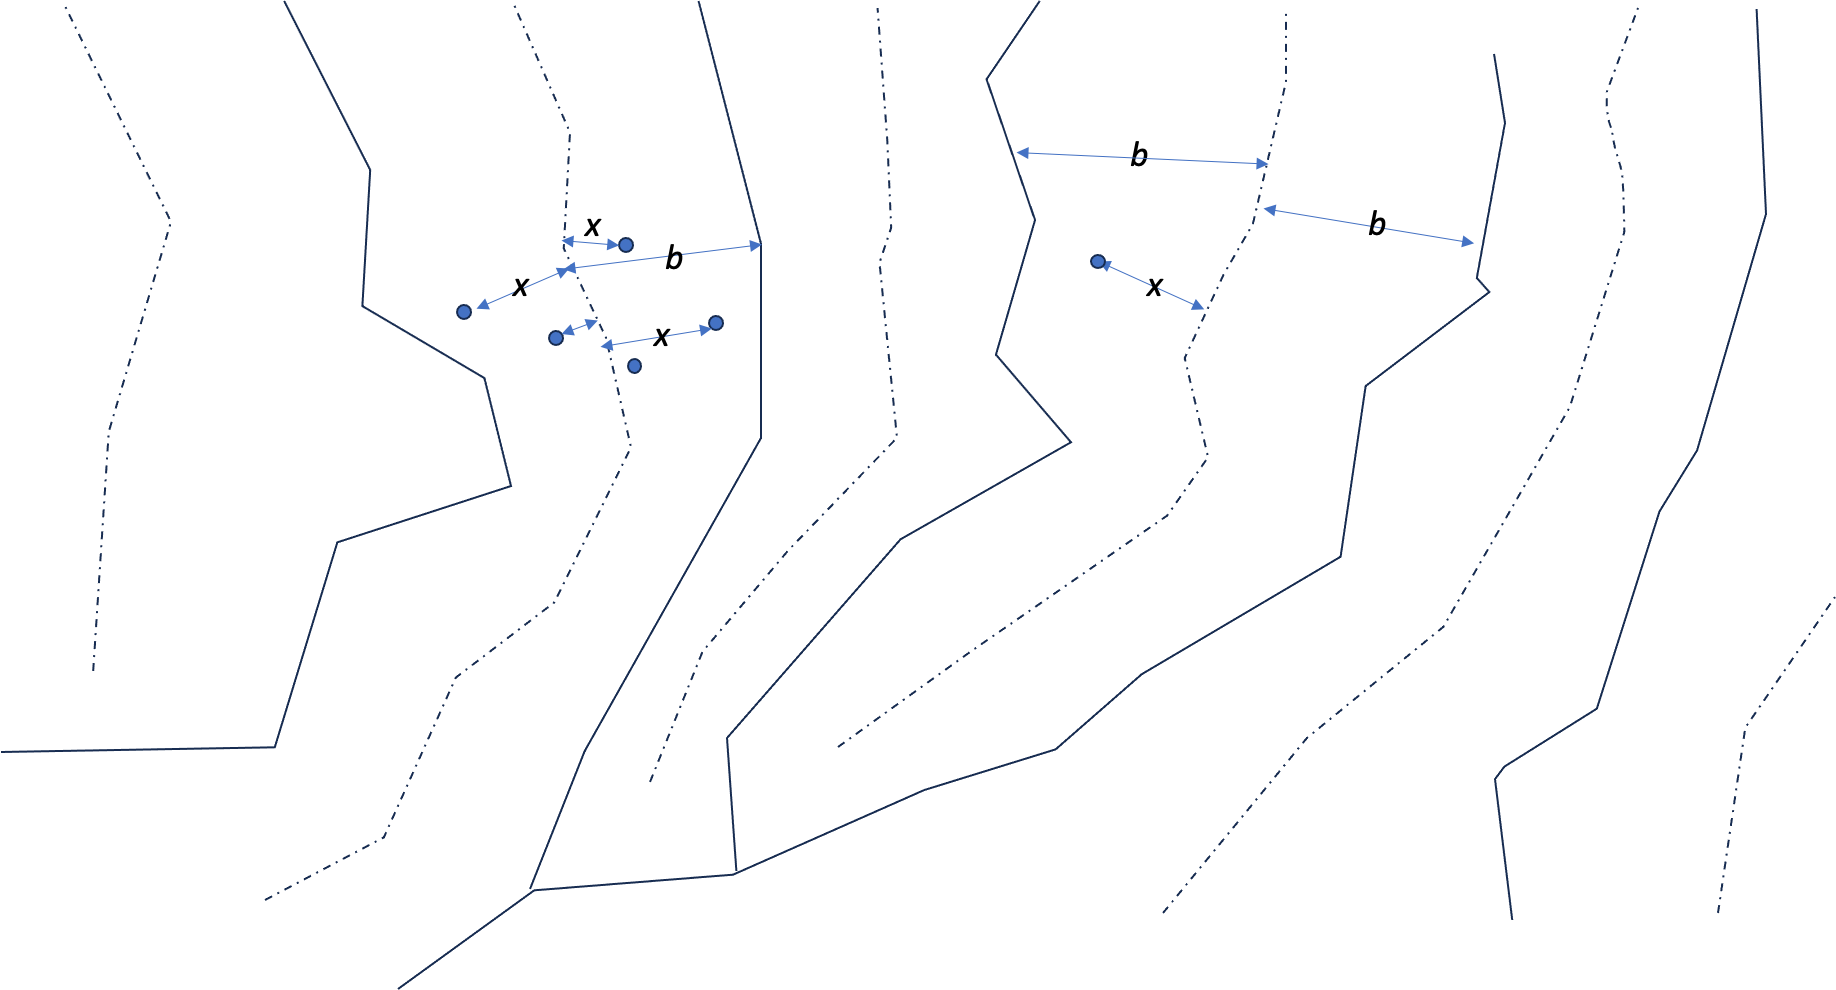
\includegraphics[width=0.8\textwidth]{../../images/waerlopen}

\caption{\label{fig:Denkbeeldig-oppervlaktestelsel}Denkbeeldig oppervlaktestelsel
waterscheiding (streepjeslijn) met waarnemingsputten }

\end{figure}

Zoals hieronder wordt afgeleid kan de weerstand van de waterlopen
vervangen worden door een equivalente vlakdekkende weerstandslaag
met weerstand $c=wL$. We kunnen vervolgens de spreidingslengte berekenen
via $\lambda=\sqrt{kDc}=\sqrt{kDwL}$. De benodigde factor $Lw$ volgt
dus direct uit de veldgegevens. Verderop zal blijken dat de situatie
met afzonderlijke open waterlopen nauwelijks afwijkt van het resultaat
waarin de waterlopen zijn vervangen door een toplaag met weerstand
$c=Lw$ mits $\lambda>L$. Voor veilige toepassing kunnen we $\lambda$
dus altijd minimaal gelijk aan $L$ aanhouden in de toe te passen
formules voor semi-spanningswater, nl. die van De Glee en Hantush.
De Glee is de stationaire versie van Hantush, dus na voldoende lange
tijd leveren beide formules hetzelfde resultaat.

Het voordeel van het (verantwoord) gebruik van de formules voor semi-spanningssituaties
in omstandigheden waarin discrete open waterlopen voorhanden zijn,
is dat de bijdragen van andere onttrekkingen zonder meer gesuperponeerd
(opgeteld) mogen worden. In het geval dat andere reeds vergunde onttrekkingen
van wat voor soort dan ook in de wijdere omgeving van de geplande
ingreep reeds aanwezig zijn, kunnen die in de berekeningen worden
meegenomen om zo het cumulatieve effect te bepalen van wat reeds is
vergund.

Een tweede voordeel van het gebruik van de formule van Hantush is
dat de duur van een onttrekking direct in de formule kan worden meegenomen,
hoe lang of kort die ook moge zijn; ook wanneer een vergunning verlengd
wordt, kan de totale duur vanaf de het verlenen van de oorspronkelijke
vergunning worden ingevuld. Uiteraard zal de uitkomst dan in de regel
gelijk zijn aan de stationaire einduitkomst, maar dat doet niets af
aan het principe.

De Glee:

\[
\Delta\phi\left(r\right)=\frac{Q}{2\pi kD}K_{0}\left(\frac{r}{\lambda}\right)
\]

Hantush

\[
\Delta\phi\left(r,t\right)=\frac{Q}{4\pi kD}\text{W}\left(u,\frac{r}{\lambda}\right),\;r=\frac{r^{2}S}{4kDt}
\]

Met $S$ de bergingscoëfficiënt en $\text{W\ensuremath{\left(u,\rho\right)}}$
De besselfunctie $K_{0}$ in De Glee's formule is een standaardfunctie;
de putformule van Hantush's kan gemakkelijk worden berekend.

\section{Vervanging van sloten door een vlakdekkende weerstandslaag}

De weerstand $c$ {[}d{]} van de vlakdekkende laag ter vervanging
de weerstand $w$ {[}d/m{]} van de sloten is niet gelijk aan de drainageweerstand
$c_{dr}$. Hij is namelijk gedefinieerd als de laag die bij een uniforme
onttrekking of infiltratie hetzelfde stijghoogteverlies veroorzaakt
als dezelfde totale onttrekking veroorzaakt over de slootweerstand.
Dus, stel we hebben een uniforme infiltratie gelijk aan het neerslagoverschot
$N$ {[}m/d{]} dan geeft de weerstandslaag met weerstand $c$ {[}d{]}
een stijghoogteverlies $\Delta\phi$ {[}m{]} van

\[
\Delta\phi=Nc
\]

En met slootafstand $L$ hebben we

\[
\Delta\phi=NLw
\]

En dus

\[
c=wL
\]


\section{Model voor een vlakke doorsnede}

We zullen de voorgestelde methode, vervanging van sloten door een
vlakdekkende weerstandslaag, illustreren aan de hand van een numeriek
eindige differentie model. Voor het gemak nemen we hiervoor een 1D
doorsnede, die met 10 km lengte lang genoeg is om geen invloed van
de modelranden te ondervinden. Dit model heeft ruim voldoende cellen
in de $x$-richting om de verlaging in detail te berekenen. In de
$y$-richting bestaat het model uit twee rijen die beide 1 m dik zijn.
In de eerste rij wordt de situatie met de individuele sloten geïmplementeerd,
met elk een slootweerstand $w$ {[}d/m{]}, en in de tweede rij wordt
het model geïmplementeerd voor de situatie zonder sloten maar met
een uniforme weerstand $c$ {[}d{]}. De twee rijen worden volledig
van elkaar gescheiden door de doorlatendheid in $y$-richting oneindig
groot te maken. Het model bestaat voorts uit slechts twee lagen, maar
er kunnen altijd willekeurig veel lagen aan worden toegevoegd. De
bovenste laag in de eerste rij (het eerste doorsnedemodel) bevat de
sloten. De cellen tussen de sloten zijn ondoorlatend. De tweede laag
stelt het watervoerend pakket voor. De eerste laag in de tweede rij
(model met de semi-permeabele toplaag) doet dienst als weerstandslaag.

Het is zaak om beide modellen volledig consistent met elkaar te maken.
Daartoe passen we bovenstaande redenering toe. Voor de weerstandslaag
is dat het meest eenvoudig. De verticale weerstand wordt vertaald
naar de verticale doorlatendheid van de toplaag. Hierbij moet worden
bedacht dat het ,,water'' in het model stroomt tussen de centra
van de modelcellen, de rekenpunten. De verticale stroming vanuit de
toplaag is derhalve over de halve dikte van de toplaag onderweg voordat
het in het watervoerende pakket aankomt. Daarna stroomt het nog door
de halve dikte van het watervoerend pakket voordat het rekenpunt wordt
bereikt. Het gaat ons om de stroming door de weerstandslaag. Dus de
verticale doorlatendheid in deze weerstandslaag moet voldoen aan

\[
N=\Delta\phi\frac{k_{z}}{0.5\Delta z}=\frac{\Delta\phi}{c}
\]

zodat de volgende verticale doorlatendheid moet worden gebruikt in
de toplaag

\[
k_{z}=\frac{\Delta z}{2c}
\]

Voor het model met de sloten ligt de zaak iets ingewikkelder. Het
blijkt dat de doorlatendheid van de cellen van de sloten behoorlijk
hoog moet zijn om de vereiste hoeveelheid water door te laten bij
hetzelfde stijghoogteverschil $\Delta\phi$. Hierdoor gaat de stromingsweerstand
vanaf de onderzijde van de toplaag met sloot tot het rekenpunt in
het midden van het watervoerende pakket een aanzienlijke bijdrage
leveren aan de totale weerstand. We zullen deze weerstand dan ook
expliciet moeten meenemen. We hebben het volgende verband tussen slootafvoer
namelijk neerslagoverschot $N$ {[}m/d{]} maar breedte $L$ van het
intrekgebied (afstand tussen de waterlopen) en slootweerstand $w$

\[
NL=\frac{\Delta\phi}{w}
\]

Vanwege de verticale stroming door de halve dikte van de twee lagen
in serie, geldt

\[
w=w_{1}+w_{2}=\frac{1}{k_{z1}}\frac{0.5\Delta z_{1}}{\Delta x}+\frac{1}{k_{z2}}\frac{0.5\Delta z_{2}}{\Delta x}
\]

Hierin is $w_{1}$ de weerstand in de bovenste modellaag en $w_{2}$
die in de laag daaronder. Deze weerstand is evenredig met de doorstroomde
laagdikte dikte $0.5\Delta z_{1}$ resp. $0.5\Delta z_{2}$, omgekeerd
evenredig met de celbreedte $\Delta x$ en omgekeerd evenredig met
de verticale doorlatendheid $k_{z1}$ resp. $k_{z2}$.

We gaan in het model de verticale doorlatendheid van de toplaag met
de sloten aanpassen, maar laten die van de laag daaronder, het watervoerende
pakket, ongemoeid. Hiermee ligt $w_{2}$ vast, terwijl ook $w$ gegeven
was. Dus

\[
w_{2}=\frac{1}{2k_{z2}}\frac{\Delta z_{2}}{\Delta x}
\]

en

\[
w=\frac{1}{2k_{z1}}\frac{\Delta z_{1}}{\Delta x}+w_{2}
\]

\[
k_{z1}=\frac{1}{2\left(w-w_{2}\right)}\frac{\Delta z_{1}}{\Delta x}
\]

In theorie zou de factor $w-w_{2}$ gelijk aan nul kunnen worden.
We kunnen dit in ons model ondervangen door in dat geval voor $w-w_{2}$
een kleine waarde te gebruiken. Negatieve waarden zijn ook mogelijk
wanneer $w_{1}>w$. Dat is het geval wanneer de verticale weerstand
over de halve dikte van de tweede modellaag groter is dan de slootweerstand.
Dit betekent alleen dat we de hoeveelheid water $NL$ niet in de sloot
kwijt kunnen bij deze slootafstand. Het model trekt zich hier niets
van aan een rekent desnoods gewoon met een negatieve verticale doorlatendheid
in de toplaag. Het lijkt verstandig om dit te signaleren en de eigenschappen
van de doorsnede in dat geval eerst fysisch realistisch te maken,
want dat is hetgeen een negatieve $k_{z1}$ signaleert.

\section{Voorbeeld}

Fig. \ref{fig:Verlaging-in-eendimensionaal} geeft de verlaging berekend
met individuele sloten met weerstand $w$ {[}d/m{]} en equivalente
uniforme drainageweerstand $c=Lw$ {[}d{]} (zie de titels in fig.
\ref{fig:Verlaging-in-eendimensionaal}voor de gebruikte waarden,
inclusief $\lambda$). De sloten liggen $L=500$ m uit elkaar en zijn
ook in \ref{fig:Verlaging-in-eendimensionaal} aangegeven. $kD=250$
m$^{2}$/d. Daar $c=Lw$ geeft een kleine slootweerstand ook een kleine
drainageweerstand en daarmee een kleine spreidingslengte $\lambda$.
Omdat de $x$-as van de plaatjes is beperkt tot -$3\lambda\le x\le3\lambda$
bij een veel langere rekenas volgens $-5000\le x\le5000$ tonen de
verschillende plaatjes in fig.\ref{fig:Verlaging-in-eendimensionaal}
een meer of minder ingezoomd deel van de $x$-as.

\begin{figure}[H]
\centering

\includegraphics[width=1\textwidth]{/Users/Theo/Entiteiten/Hygea/2022-AGT/Coding/images/drawdown_xsec_4xw}

\caption{\label{fig:Verlaging-in-eendimensionaal}Verlaging in eendimensionale
doorsnede. Blauw de oplossing met voeding via individuele waterlopen
met intree/uittreeweerstand $w$ {[}d/m{]}. Rood de equivalente oplossing
waarin de waterlopen zijn vervangen door een uniforme drainageweerstand
$c$ {[}d{]} De $x$-as van de plaatjes is begrensd tussen $-3\lambda<x<3\lambda$,
maar de reken-$x$-as is $-5000<x<5000$.}

\end{figure}

De figuur laat zien dat met name bij kleine $\lambda$, in concreto
$\lambda<L$, er een aanmerkelijk verschil is tussen beide situaties.
Hoe kleiner de $\lambda$ hoe meer de individuele sloten het verlagingsbeeld
bepalen. Pas bij $\lambda$ groter dan zeg $L$ ontlopen de rekenwijzen
elkaar nauwelijks meer.

In dit ééndimensionale voorbeeld is het stijghoogteverloop tussen
de individuele sloten lineair, wat goed in de figuren tot uiting komt.
De verlaging nabij de onttrekking is dan ook een stuk kleiner dan
in de berekening met een uniforme drainageweerstand.

Behalve de numeriek berekende verlaging is in fig.\ref{fig:Verlaging-in-eendimensionaal}
ook de analytisch berekende verlaging opgenomen en met markers aangegeven.
Die van de doorsnede met sloten is van de ene sloot naar de andere
gerekend met het constante debiet ertussen uit het numerieke model

\[
\phi_{i}=\phi_{i-1}-\frac{Q_{x}}{kD}\left(x_{i}-x_{i-1}\right)
\]

De analytische verlaging in de doorsnede met weerstandbiedende toplaag
is

\[
\phi_{x_{w}}-\phi_{x}=-\frac{\lambda}{kD}\frac{Q}{2}e^{-\left|x-x_{w}\right|/\lambda}
\]

De figuren laten zien dat de numerieke en analytische resultaten nauwkeurig
met elkaar overeenkomen. De figuren laten verder zien dat wanneer
de slootafstand groter is dan de spreidingslengte van de equivalente
vlakdekkende toplaag, de uitkomsten van beide rekenmethoden nagenoeg
niet meer van elkaar zijn te onderscheiden. Voor kleinere spreidingslengten
wordt toepassing problematisch en des te meer naarmate de verhouding
$\lambda/L$ meer onder de 1 uitkomt.

\[
\lambda=\sqrt{kDc}=\sqrt{kDwL}
\]

\[
\frac{\lambda}{L}=\sqrt{kD\frac{w}{L}}
\]

Dus voor de gegevens in de figuur met waarden

\[
w=[0.25,\;0.5,\;1,\;2]\;\text{[d/m]}
\]

\[
\frac{\lambda}{L}=[0.35,\;0.5,\;0.71,\;1]
\]


\section{Driedimensionaal model}

We kunnen hetzelfde voorbeeld doorrekenen voor een 3D model met een
(put)onttrekking in het centrum. Ook dit doen we door twee modellen
tegelijkertijd uit de rekenen. Het eerste model heeft individuele
sloten in $y$-richting op afstand $L$ uit elkaar en met slootweerstand
$w$ {[}d/m{]}. Het tweede model heeft in plaats van de sloten een
equivalente vlakdekkende weerstandslaag met weerstand $c$, waarin,
net als in de sloten, het peil wordt aangehouden. Het model heeft
nu een vierkant netwerk met cellen en twee lagen. De lijn $y=0$ fungeert
als scheiding van beide modellen, die elk een halfvlak beslaan met
een put aan de rand. Het netwerk is fijn in de $x$-richting, het
verfijnt steeds tot ca. 1 m celbreedte bij elke sloot. Het netwerk
in $y$-richting wordt logaritmisch grover wordt met de afstand tot
de lijn $y=0$. De rij aan weerszijden van de scheiding ($y=0)$ heeft
een breedte van ongeveer $1$m. De scheiding zelf in een rij van modelcellen
2 mm breed, 1 mm aan elke kant van de $y=0$ lijn, waarin de cellen
op inactief zijn gezet en daarom niet meedoen.

Het model heeft twee lagen waarvan de bovenste 2 m dik is en de onderste
25 m. De stijghoogte in het model met de sloten wordt alleen op nul
vastgezet voor de slootcellen in de toplaag. In het model met de equivalente
weerstandslaag wordt de stijghoogte in alle cellen van de toplaag
op nul gezet. De horizontale doorlatendheid in de toplaag wordt in
beide modellen op nul vastgehouden. In de toplaag is dus alleen verticale
stroming mogelijk.

Op deze wijze ingericht zijn de hier beschreven twee modellen de 3D-evenknie
van de doorsnedemodellen die hierboven zijn uitgewerkt, behalve de
de put: De onttrekking $Q_{w}$ door de put heeft nu dimensie m$^{3}$/d
en het water stroomt er radiaal naar toe, terwijl de onttrekking $Q_{w}$
in het doorsnedemodel een verticale sleufonttrekking was met dimensie
m$^{2}$/d.

De slootweerstand $w$ geldt voor een oneindig lange sloot (net als
in de doorsnede) en volgt uit

\[
w=\frac{\Delta\phi}{Q}
\]

Met $\Delta\phi$ slootpeil minus stijghoogte in de onderliggende
aquifer en $Q$ de slootonttrekking in {[}m2/d{]} oftewel {[}m$^{3}$/(d$\times$m\_sloot\_lengte){]}
Voor een cel met slootlengte $\Delta y$ geldt een totaal debiet $Q_{cel}$
{[}m$^{3}$/d{]} volgens

\[
Q_{cel}=\frac{\Delta\phi}{w_{c}}=\frac{\Delta\phi}{w}\Delta y=\left[\frac{m}{d/m}m\right]=\left[\frac{m^{3}}{d}\right]
\]

Willen we een weerstand per m$^{2}$ celoppervlak hebben, dan delen
we $Q_{cel}$ door dit oppervlak

\[
q=\frac{Q_{cel}}{\Delta x\Delta y}=\frac{\Delta\phi}{w}\frac{\Delta y}{\Delta x\Delta y}=\frac{\Delta\phi}{w\Delta x}[m/d]
\]

Met andere woorden, $w\Delta x$ {[}d/m$\times$m{]}={[}d{]} is nu
een verticale weerstand per oppervlakte-eenheid net als de $c$ {[}d{]}
van een afdekkende laag. Hiermee kan de verticale stroming door een
cel worden berekend.

\[
w\Delta x=w1\Delta x+w2\Delta x
\]

\[
Q_{v}=\frac{\Delta\phi}{w_{1}\Delta x+w_{2}\Delta x}\Delta x\Delta y=\frac{\Delta\phi}{\frac{0.5\Delta z_{1}}{k_{z1}}+\frac{0.5\Delta z_{2}}{k_{z2}}}\Delta x\Delta y
\]

\[
w_{1}\Delta x+w_{2}\Delta x=\frac{0.5\Delta z_{1}}{k_{z1}}+\frac{0.5\Delta z_{2}}{k_{z2}}
\]

\[
w_{2}=\frac{1}{k_{z2}}\frac{\Delta z_{2}}{2\Delta x}
\]

We zoeken $k_{z1}$ omdat we $k_{z2}$ in tact laten

\[
\left(w-w_{1}\right)\Delta x=\frac{1}{k_{z1}}\frac{\Delta z_{1}}{2\Delta x}
\]

\[
k_{z1}=\frac{1}{2\left(w-w_{2}\right)}\frac{\Delta z_{1}}{\Delta x}
\]

Dit is hetzelfde als in het doorsnede model. En dat is ook logisch.

\section{Voorbeeld onttrekking in gebied met evenwijdige open leidingen}

Fig. \ref{fig:Verlaging-door-een-put} toont het resultaat van de
berekening. In blauw is de verlaging weergegeven wanneer de voeding
van het pakket als gevolg van de onttrekking geheel plaats vindt via
sloten met gegeven slootweerstand $w$ {[}d/m{]}. In rood is de verlaging
weergegeven wanneer de voeding plaats vindt via een vlakdekkende semi-permeabele
toplaag met weerstand $c$ {[}d{]}. Met rode cirkels is de analytisch
berekende verlaging getekend volgens De Glee:

\[
\Delta\phi=\frac{Q_{w}}{2\pi kD}K_{0}\left(\frac{r}{\lambda}\right)
\]

De sloten lopen loodrecht op de hier getekende doorsnede en liggen
500 m uit elkaar. Net als het geval was bij de resultaten van de verlaging
door een verticale oneindig lange lijnonttrekking in de hiervoor uitgewerkte
vlakke doorsnede, blijkt dat de uitkomsten verschillen voor $\lambda<L$
voor grotere afstanden is het verschil tussen de uitkomsten volstrekt
verwaarloosbaar.

\begin{figure}[H]
\centering

\includegraphics[width=1\textwidth]{/Users/Theo/Entiteiten/Hygea/2022-AGT/Coding/images/drawdown_3D_4xw}

\caption{\label{fig:Verlaging-door-een-put} Blauw: Verlaging door een onttrekkingsbron
wanneer de voeding van het pakket geheel via afzonderlijke waterlopen
plaats vindt (hier 500 m uiteen). Rood: Wanneer de voeding van het
watervoerende pakket plaats vindt via een equivalente vlakdekkende
equivalente semi-permeabele toplaag.}

\end{figure}


\section{Test met een regionaal model}

We zullen nu de proef op de som nemen en de vereenvoudiging toepassen
op een regionaal model. Het model beslaat een willekeurig stuk van
België met een karakteristiek stelsel oppervlaktewateren voornamelijk
bestaande uit beken. We gaan uit van een homogeen freatisch pakket
met uniforme dikte en geven het oppervlaktewater overal dezelfde radiale
weerstand. We modelleren het gebied opnieuw met slechts twee modellagen.
Alle cellen van de eerste laag krijgen $k_{x}=k_{y}=0$. De verticale
doorlatendheid wordt niet veranderd behalve bij de cellen die oppervlaktewater
bevatten. Voor die cellen wordt de verticale doorlatendheid zodanig
aangepast dat deze precies de radiale weerstand van dat oppervlaktewater
binnen de cel simuleert. De cellen met oppervlaktewater krijgen een
vaste stijghoogte gelijk aan nul. Neerslag wordt niet toegepast. De
beoogde ingreep, een onttrekking wordt aan de tweede laag opgelegd.
Dit is gelijk het enige dat in de tweede laag plaats vindt.

Dit model wordt vergeleken met een model waarin het oppervlaktewater
is vervangen door een equivalente semi-permeabele toplaag. De weerstand
daarvan wordt consistent gemaakt met die van het stelsel aan oppervlaktewater.
De stijghoogte in deze toplaag wordt vastgezet op 0. Vervolgens wordt
in de tweede laag de beoogde ingreep aangebracht op dezelfde manier
als hiervoor.

Beide modellen worden gedraaid en de resultaten worden daarna met
elkaar vergeleken.

\[
\frac{Q}{\Delta\phi}=\frac{L}{w}=\frac{L}{w_{1}+w_{2}}=\frac{1}{\frac{w_{1}}{L}+\frac{w_{2}}{L}}=\frac{1}{c_{1}+c_{2}}=\frac{1}{\frac{2\Delta z_{1}}{k_{z1}}+\frac{2\Delta z_{2}}{k_{z2}}}
\]

Met $w=w_{1}+w_{2}$de totale weerstand van de sloot maar nu verdeeld
over modellaag 1 en 2 

\[
\frac{w}{L}=c_{1}+c_{2}=\frac{2\Delta z_{1}}{k_{z1}}+\frac{2\Delta z_{2}}{k_{z2}}
\]

Met gegeven laageigenschappen is $c_{2}$ bekend. $c_{2}$ is gegeven
en wordt niet aangepast. Dus resteert het aanpassen van de verticale
doorlatendheid van de eerste modellaag $k_{z1}$. Deze volgt uit

\[
\frac{w}{L}=\frac{2\Delta z_{1}}{k_{z1}}+c_{2}
\]

zodat

\[
k_{z1}=\frac{2\Delta z_{1}}{\frac{w}{L}-c_{2}};\;c_{2}=\frac{2\Delta z_{2}}{k_{z2}}
\]

De vraag is nu welke equivalente weerstand moeten we gebruiken ter
vervanging van het oppervlaktewater. In de situatie waarin het open
water was opgevat als evenwijdig, wat dat eenduidig. Die luxe gaat
met willekeurig over het gebied verdeeld oppervlaktewater natuurlijk
niet op. We moeten voor deze waarde terugvallen op een of ander met
GIS berekenbaar criterium. Een mogelijkheid is om een fijn raster
te maken met voor elke cel de afstand tot het dichtstbij zijnde oppervlaktewater.
Afb.@@@) laat het resultaat van zo'n bewerking zien. Het is een berglandschap
met uitsluitend positieve hoogtes variërend van 0 ter plaats van het
oppervlaktewater tot een maximum daartussen. Dit landschap heeft graten
als in een echt berglandschap, die waterscheidingen vormen. De hoogte
van de graat kan worden opgevat als de afstand $b$, de halve breedte
van het gebied opgespannen tussen twee meestal min of meer evenwijdige
waterlopen. Het grondwaterverloop langs een doorsnede loodrecht op
de hoogtelijnen tussen twee waterlopen zal ongeveer voldoen aan Dupuit:

\[
h-h_{0}\approx Nbw+\frac{N}{2kD}\left(b_{2}-x^{2}\right);\;\text{met \;0\ensuremath{\le}x\ensuremath{\le}b}
\]

Voor elk punt in het gebied kan $b$ uit deze rasterkaart worden bepaald
door van dat punt de naar boven te klimmen tot de graat is bereikt.
Zoals hiervoor uitgelegd is de vervangende equivalente weerstand voor
het gebied met evenwijdig oppervlaktewater op onderlinge afstand $L=2b$
gelijk aan

\[
Q=\frac{\Delta\phi}{w}=\frac{\Delta\phi}{c}L\to c=Lw
\]

Dit kunnen we ook in het ruimtelijke geval toepassen waarbij $L=2b$
uit de afstandskaart in het gebied van de ingreep. 

Fig.\ref{figAfstand-tot-het-pppervlaktewater} geeft een kaart met
de loop van oppervlaktewateren en contourlijnen van de kortste afstand
tot het oppervlaktewater. De ,,kam'' met de hoogte waarden is geel
aangegeven. De kam hoogte is de halve breedte $b$ ofwel $L/2$ overeenkomstig
de afstand $L$ tussen parallelle waterlopen. De gele lijnen geven
de grootste halve afstand tussen het lokale oppervlaktewater. Hierna
worden voorbeeldberekeningen gemaakt voor de vijf locaties die in
fig.\ref{figAfstand-tot-het-pppervlaktewater} zijn weergegeven als
witte bolletjes. Vanuit elk bolletje gaat een lijntje naar het lokale
hoogste punt (grootste afstand tot het oppervlaktewater) dit levert
de afstand $b$ (locatie is aangegeven met oranje bolletjes). Met
deze gegevens, de slootweerstand $w$ en het doorlaatvermogen kunnen
de voorbeeldberekeningen worden gemaakt. In de figuren met resultaten
van elk van de voorbeeldberekeningen zijn de rode verlagingslijnen
die de uitkomst weergeven van de berekening met het oppervlaktewater
als randvoorwaarde, terwijl de zwarte cirkelvormige verlagingslijnen
het resultaat zijn van de berekening waarin het oppervlaktewater is
vervangen door een equivalente semi-permeabele toplaag.

\begin{figure}[h]
\centering

\includegraphics[width=0.8\textwidth]{/Users/Theo/Entiteiten/Hygea/2022-AGT/Coding/images/afstand_tot_oppwater}\caption{\label{figAfstand-tot-het-pppervlaktewater}Oppervlaktewater met contourlijnen
van de afstand tot het oppervlaktewater. De ,,kam'' tussen het oppervlaktewater
is geel aangeduid. De afbeelding toont een vijftal locaties waar een
ingreep wordt gesimuleerd (witte bollen). De bij deze punten behorende
$b=L/2$ is met een gele bol aangegeven.}

\end{figure}

De procedure om de invloed of reikwijdte van een lokale ingreep in
het grondwatersysteem te berekenen zou als volgt zijn:
\begin{enumerate}
\item Bepaal de locatie.
\item Ga vanaf deze locatie ,,bergop'' tot de kam.
\item Gebruik deze kamhoogte als $L$
\item Bereken de equivalente weerstand uit $c=Lw$ met $w$ de radiale slootweerstand
eventueel vermeerderd met de bodemslibweerstand.
\item Bereken analytisch met De Glee of Hantush de verlagingen en de verlagingscontouren.
\end{enumerate}

\section{Voorbeelden}

De volgende figuren geen de resultaten van de verlagingsberekening
voor een onttrekking van $Q=3000$ m3/d op achtereenvolgens vijf verschillende
locaties in hetzelfde gebied. De locaties zijn dezelfde als de witte
bolletjes in fig.\ref{figAfstand-tot-het-pppervlaktewater}. De locaties
zijn zo gekozen dat de plek ten opzichte van het oppervlak voor elk
punt wezenlijk anders is. De rode contourlijnen geven de verlaging
met het oppervlaktewater als randvoorwaarde, waarbij al het oppervlaktewater
dezelfde (radiale) weerstand $w$ heeft zoals aangegeven in de kop
van de figuur. De zwarte contourlijnen geven de berekende verlaging
weer waarbij het oppervlaktewater is vervangen door een toplaag met
equivalente weerstand $c$ ook aangegeven in de op van elke figuur.
Deze weerstand $c=2bw$ hangt af van de afstand tussen het oppervlaktewater
(halve afstand $b$ is de waarde van het corresponderende gele bolletje
in fig.\ref{figAfstand-tot-het-pppervlaktewater}). Deze afstand varieert
feitelijk over het gebied maar de waarde voor het onttrekkingspunt
is aangehouden. De verlagingen volgens De Glee zijn gecheckt en komen
strak overeen met de zwarte contourlijnen, maar zijn om die reden
hier niet getekend.

In fig.\ref{fig:192300-194100} blijkt de verlaging van de berekening
met oppervlaktewater redelijk overeen te komen met die volgens De
Glee, behalve in het zuidwesten, waar gewoon weinig oppervlaktewater
aanwezig is om de verlaging te dempen, daar is de verlaging groter
dan volgens De Glee..

\begin{figure}[h]
\centering

\includegraphics[width=0.8\textwidth]{/Users/Theo/Entiteiten/Hygea/2022-AGT/Coding/images/fdm_de_Glee_xy_192300_194100}

\caption{\label{fig:192300-194100}Verlagingen rond punt $xy$=(192300,194100)}

\end{figure}

In fig.\ref{fig:193400-198550} is de reikwijdte volgens de analytische
formule van De Glee in het noordwesten veel groter dan de berekening
met de sloten. Dit wordt duidelijk veroorzaakt door een dichter stelsel
oppervlaktewater ten noordwesten van de onttrekking. De $\lambda$
waarde is relatief groot door de grote afstand tussen het oppervlaktewater
rond de onttrekking.

\begin{figure}[h]
\centering

\includegraphics[width=0.8\textwidth]{/Users/Theo/Entiteiten/Hygea/2022-AGT/Coding/images/fdm_de_Glee_xy_193400_198550}

\caption{\label{fig:193400-198550}Verlagingen rond punt $xy$=(193400,198550)}

\end{figure}

In fig.\ref{fig:193500-196200} is de reikwijdte volgens De Glee in
het noorden duidelijk groter dan die van de berekening met oppervlaktewater.
De reden is dat in het noorden de dichtheid van het oppervlaktewater
groter is, terwijl de $\lambda$ hier juist groot is door de grote
afstand tussen het oppervlaktewater in het stroomgebied waar de onttrekking
zich toevallig in bevindt $b=800$, $\lambda=800$ m.

\begin{figure}[h]
\centering

\includegraphics[width=0.8\textwidth]{/Users/Theo/Entiteiten/Hygea/2022-AGT/Coding/images/fdm_de_Glee_xy_193500_196200}

\caption{\label{fig:193500-196200}Verlagingen rond punt $xy$=(193500,196200)}

\end{figure}

In fig.\ref{fig:195000-196500} is het invloedsgebied volgens De Glee
groter dan met het oppervlaktewater als randvoorwaarde. De oorzaak
hiervan is de ligging van de onttrekking vlakbij oppervlaktewater,
dat de reikwijdte verkleint terwijl de reikwijdte volgens De Glee
afhangt van de $\lambda$-waarde die juist groot is door de grote
afstand tussen het oppervlaktewater in het gebied waar de onttrekking
zich bevindt $\left(2b=1200,\;\lambda\approx700\right)$ m. en 

\begin{figure}[h]
\centering

\includegraphics[width=0.8\textwidth]{/Users/Theo/Entiteiten/Hygea/2022-AGT/Coding/images/fdm_de_Glee_xy_195000_196500}

\caption{\label{fig:195000-196500}Verlagingen rond punt $xy$=(195000,196500)}

\end{figure}

Fig. \ref{fig:196250-195600} is een situatie waarin de reikwijdte
van de berekening met oppervlaktewater juist groter is dan die volgens
De Glee. Dit wordt veroorzaakt door de wat geringere afstand tussen
het oppervlaktewater en dus kleinere $b$ en kleinere $\lambda$.
Maar de groter reikwijdte van de berekening met het oppervlaktewater
komt ook door een geringe dichtheid van datzelfde oppervlaktewater
in flinke delen van het beïnvloede gebied.

\begin{figure}[h]
\centering

\includegraphics[width=0.8\textwidth]{/Users/Theo/Entiteiten/Hygea/2022-AGT/Coding/images/fdm_de_Glee_xy_196250_195600}

\caption{\label{fig:196250-195600}Verlagingen rond punt $xy$=(196250,195600)}
\end{figure}

Bij de voorbeelden met parallel oppervlaktewater is geconcludeerd
dat $\lambda\ge2b$ zou moeten zijn wil de berekeningsmethode goed
werken. Zulke grote waarden worden in deze voorbeelden niet gehaald.
Zet men $\lambda=2b$, dan zijn de verlagingen die met de vervangende
semi-permeabele laag worden berekend in de meeste gevallen veel te
groot. Hieronder worden hiervan twee voorbeelden gegeven. Zij zijn
gelijk aan twee van de voorgaande voorbeelden maar met een grotere
$\lambda=2b$.

Fig.\ref{fig:193400-198550-2b} is dezelfde situatie als fig.\ref{fig:193400-198550}
maar nu met $\lambda=2b$. De berekeningen met de vervangende semi-permeabele
laag geven bij $\lambda=2b=1200$ mu veel grotere verlagingen dan
in fig.\ref{fig:193400-198550} met $\lambda\approx700$ m.

\begin{figure}[h]
\centering

\includegraphics[width=0.8\textwidth]{/Users/Theo/Entiteiten/Hygea/2022-AGT/Coding/images/fdm_de_Glee_xy_193400_198550_2b}

\caption{\label{fig:193400-198550-2b}Zelfde situatie als in fig.\ref{fig:193400-198550}
maar met $\lambda=2b=1200$ m}

\end{figure}

Fig.\ref{fig:196250-195600-2b} is dezelfde situatie als in fig.\ref{fig:196250-195600}
maar nu met $\lambda=2b=700$ m in plaats van 529 m. In dit geval
is $\lambda=2b$ zelfs wat beter. Dat komt ook omdat hier $\lambda$
en $2b$ niet ver uiteen lopen.

\begin{figure}[h]
\centering

\includegraphics[width=0.8\textwidth]{/Users/Theo/Entiteiten/Hygea/2022-AGT/Coding/images/fdm_de_Glee_xy_196250_195600_2b}

\caption{\label{fig:196250-195600-2b}Zelfde situatie als in fig.\ref{fig:196250-195600}
maar met $c=2b$}

\end{figure}


\section{Conclusies}

In situaties met parallel oppervlaktewater lijkt het acceptabel om
voor de berekening van de verlaging en zijn reikwijdte de sloten te
vervangen door een equivalente semi-permeabele toplaag onder voorwaarde
dat $\lambda/L>1$. Voor zeer grote afstanden van de onttrekking is
er hoe dan ook weinig verschil tussen de uitkomsten. De afwijkingen
concentreren zich rond de onttrekking. Dit geldt zowel voor de eendimensionale
situatie, dat wil zeggen een verticale vlakke doorsnede met lijnonttrekking,
als in de driedimensionale situatie met een brononttrekking.

Bij een min of meer willekeurige ruimtelijke en spaarzame verdeling
van het oppervlaktewater over het gebied zijn er duidelijke verschillen
tussen de uitkomsten van de berekening met het oppervlaktewater als
randvoorwaarde en de uitkomsten van de berekening waarbij het oppervlaktewater
is vervangen door een ,,equivalente'' uniforme weerstandslaag. De
verschillen hangen sterk af van de daadwerkelijke verdeling van het
oppervlaktewater over het gebied, zoals blijkt uit de vijf voorbeelden
waarbij de onttrekking steeds op een (significant) andere plek in
het gebied werd geplaatst.

De equivalente weerstand van de vervangende toplaag wordt berekend
op basis van slootweerstand en afstand tussen het oppervlaktewater
in het gebied waar de onttrekking zich bevindt. Deze afstand kan van
plaats tot plaats sterk verschillen waardoor er verschillen ontstaan
tussen de twee rekenmethoden. De rekenmethodes zijn eenduidig maar
waar de verschillen optreden is niet a priori te zeggen. De berekening
met de vervangende semi-permeabele toplaag is in het algemeen minder
accuraat tenzij de spreidingslengte $\lambda$ groter dan dan de afstand
tussen het oppervlaktewater $2b$. Dat is hij echter in dit gebied
nooit. De vervangende weerstand $c=2bw$ en hangt behalve van de $b$
ook direct af van de grootte van de radiale weerstand $w$. De waarde
$w$ die in deze vijf voorbeeldberekeningen is toegepast is 2 d/m,
en was de hoogste waarde toegepast in fig.\ref{fig:Verlaging-door-een-put}.
Bij deze waarde is de $\lambda$ in dit gebied kleiner dan $2b$ waardoor
de equivalente scheidingslaag minder goed werkt. Dit zal vermoedelijk
altijd zo zijn in gebieden met een grote afstand tussen het oppervlaktewater.

De ,,eis'' $\lambda\ge2b$ kan leiden tot een keuze voor $\lambda=2b$
ongeacht wat $c=2bw$ feitelijk is. De laatste twee voorbeelden illustreren
dat dit in zijn algemeenheid geen goed idee is. De berekeningen met
equivalenten semi-permeabele laag kunnen dan veel te grote verlagingen
berekenen, hoewel dat niet altijd het geval blijkt. Dit maakt de berekeningswijze
onbetrouwbaar en is dus af te raden.

De hier uitgewerkte aanpak kan werken, en is dan eenvoudig, maar blijft
verre van perfect. In hoeverre deze voor de Voortoets acceptabel zal
zijn moet in breder verband worden besloten.
\begin{thebibliography}{Kruseman en De Ridder (1994)}
\bibitem[Bruggeman (1999)]{Brug99}Bruggeman G.A. (1999) Analyical
Solutions of Geohydrological Problems. Elsevier + RIVM, Developments
in Water Science no. 46. ISBN 0 444 81829 4, 959p.

\bibitem[Ernst (1962)]{Ernst62}Ernst, L.F. (1962) Grondwaterstromingen
in de verzadigde zone en hun berekening bij de aanwezigheid van open
leidingen. Pudoc, Publ. 67.15, Wageningen. 189pp.

\bibitem[Huisman (1972)]{Huis72}Huisman, L. (1972) Groundwater Recovery.
MacMillan, SBN 333 09870 6. Pitman Press, Bath. 336p.

\bibitem[Kruseman en De Ridder (1994)]{KR94}Kruseman, G.P. and N.A.
de Ridder (1994) Analysis and Evaluation of Pumping Test Data. ISBN
90 70754207. ILRI publication 47. 376.

\end{thebibliography}

\end{document}
